% !TEX TS-program = lualatex
% !TEX encoding = UTF-8 Unicode		

\documentclass[12pt, letterpaper]{article}

%%BIBLIOGRAPHY- This uses biber/biblatex to generate bibliographies according to the 
%%Unified Style Sheet for Linguistics
\usepackage[main=american, german]{babel}% Recommended
\usepackage{csquotes}% Recommended
\usepackage[backend=biber,
		style=unified,
		maxcitenames=3,
		maxbibnames=99,
		natbib,
		url=false]{biblatex}
\addbibresource{link.bib}
\setcounter{biburlnumpenalty}{100}  % allow URL breaks at numbers
%\setcounter{biburlucpenalty}{100}   % allow URL breaks at uppercase letters
%\setcounter{biburllcpenalty}{100}   % allow URL breaks at lowercase letters

%%TYPOLOGY
\usepackage[svgnames]{xcolor} % Specify colors by their 'svgnames', for a full list of all colors available see here: http://www.latextemplates.com/svgnames-colors
%\usepackage[compact]{titlesec}
%\titleformat{\section}[runin]{\normalfont\bfseries}{\thesection.}{.5em}{}[.]
%\titleformat{\subsection}[runin]{\normalfont\scshape}{\thesubsection}{.5em}{}[.]
\usepackage[hmargin=1in,vmargin=1in]{geometry}  %Margins          
\usepackage{graphicx}	%Inserting graphics, pictures, images 		
\usepackage{stackengine} %Package to allow text above or below other text, Also helpful for HG weights 
\usepackage{fontspec} %Selection of fonts must be ran in XeLaTeX or LuaLaTeX
\usepackage{amssymb} %Math symbols
\usepackage{amsmath} % Mathematical enhancements for LaTeX
\usepackage{setspace} %Linespacing
\usepackage{multicol} %Multicolumn text
\usepackage{enumitem} %Allows for continuous numbering of lists over examples, etc.
\usepackage{multirow} %Useful for combining cells in tablesbrew 
\usepackage{booktabs}
\usepackage{hanging}
\usepackage{fancyhdr} %Allows for the 
\pagestyle{fancy}
\fancyhead[L]{\textit{QP Handout}} 
\fancyhead[R]{\textit{\today}} 
\fancyfoot[L,R]{} 
\fancyfoot[C]{\thepage} 
\renewcommand{\headrulewidth}{0.4pt}
\setlength{\headheight}{14.5pt} % ...at least 14.49998pt
% \usepackage{fourier} % This allows for the use of certain wingdings like bombs, frowns, etc.
% \usepackage{fourier-orns} %More useful symbols like bombs and jolly-roger, mostly for OT
\usepackage[colorlinks,allcolors={black},urlcolor={blue}]{hyperref} %allows for hyperlinks and pdf bookmarks
% \usepackage{url} %allows for urls
% \def\UrlBreaks{\do\/\do-} %allows for urls to be broken up
\usepackage[normalem]{ulem} %strike out text. Handy for syntax
\usepackage{tcolorbox}
\usepackage{datetime2}

%%FONTS
\setmainfont{Libertinus Serif}
\setsansfont{Libertinus Sans}
\setmonofont[Scale=MatchLowercase]{Libertinus Mono}

%%PACKAGES FOR LINGUISTICS
%\usepackage{OTtablx} %Generating tableaux with using TIPA
\usepackage[noipa]{OTtablx} % Use this one generating tableaux without using TIPA
%\usepackage[notipa]{ot-tableau} % Another tableau drawing packing use for posters.
% \usepackage{linguex} % Linguistic examples
% \usepackage{langsci-linguex} % Linguistic examples
\usepackage{langsci-gb4e} % Language Science Press' modification of gb4e
% \usepackage{langsci-avm} % Language Science Press' AVM package
\usepackage{tikz} % Drawing Hasse diagrams
% \usepackage{pst-asr} % Drawing autosegmental features
\usepackage{pstricks} % required for pst-asr, OTtablx, pst-jtree.
% \usepackage{pst-jtree} 	% Syntax tree draawing software
% \usepackage{tikz-qtree}	% Another syntax tree drawing software. Uses bracket notation.
\usepackage[linguistics]{forest}	% Another syntax tree drawing software. Uses bracket notation.
% \usepackage{ling-macros} % Various linguistic macros. Does not work with linguex.
% \usepackage{covington} % Another linguistic examples package.
\usepackage{leipzig} %	Offers support for Leipzig Glossing Rules

%%LEIPZIG GLOSSING FOR ZAPOTEC
\newleipzig{el}{el}{elder}	% Elder pronouns
\newleipzig{hu}{hu}{human}	% Human pronouns
\newleipzig{an}{an}{animate}	% Animate pronouns
\newleipzig{in}{in}{inanimate}	% Inanimate pronouns
\newleipzig{pot}{pot}{potential}	% Potential Aspect
\newleipzig{cont}{cont}{continuative}	% Continuative Aspect
% \newleipzig{pot}{pot}{potential}	% Potential Aspect
\newleipzig{stat}{stat}{stative}	% Potential Aspect
\newleipzig{and}{and}{andative}	% Andative Aspect
\newleipzig{ven}{ven}{venative}	% Venative Aspect
% \newleipzig{res}{res}{restitutive}	% Restitutive Aspect
\newleipzig{rep}{rep}{repetitive}	% Repetitive Aspect

%%TITLE INFORMATION
\title{TITLE}
\author{Mykel Loren Brinkerhoff}
\date{\today}

%%MACROS
\newcommand{\sub}[1]{\textsubscript{#1}}
\newcommand{\supr}[1]{\textsuperscript{#1}}
\providecommand{\lsptoprule}{\midrule\toprule}
\providecommand{\lspbottomrule}{\bottomrule\midrule}
\newcommand{\fittable}[1]{\resizebox{\textwidth}{!}{#1}}

\makeatletter
\renewcommand{\paragraph}{%
  \@startsection{paragraph}{4}%
  {\z@}{0ex \@plus 1ex \@minus .2ex}{-1em}%
  {\normalfont\normalsize\bfseries}%
}
\makeatother
\parindent=10pt


\begin{document}
	
%%If using linguex, need the following commands to get correct LSA style spacing
%% these have to be after  \begin{document}
	% \setlength{\Extopsep}{6pt}
	% \setlength{\Exlabelsep}{9pt}		%effect of 0.4in indent from left text edge
%%
	
%% Line spacing setting. Comment out the line spacing you do not need. Comment out all if you want single spacing.
%	\doublespacing
%	\onehalfspacing
	
\begin{center}
	{\Large \textbf{Tone and phonation in Santiago Laxopa Zapotec}}
	\vspace{6pt}

	Mykel Loren Brinkerhoff
\end{center}
%\maketitle
%\maketitleinst
\thispagestyle{fancy}

\tableofcontents

%------------------------------------
\section{Introduction} \label{sec:Introduction}
%------------------------------------

\begin{itemize}
	\item Most work on the interaction of tone and phonation has been based on descriptions of southeast and far east Asian languages.
	\item This lead to strong claims on the interaction between tone and phonation \citep{masicaDefiningLinguisticArea1976,thurgoodVietnameseTonogenesisRevising2002,yipTone2002,enfieldArealLinguisticsMainland2005,michaudComplexTonesEast2012,brunelleTonePhonationSoutheast2016}.
	\item Main claim from these authors is that tone and phonation are codependent. This is often referred to as a register system.  
	\begin{itemize}
		\item Meaning that we only observe certain tones with certain phonations. 
		\item Mandarin Tone 3 is always associated with creaky voice \citep{duanmuPhonologyStandardChinese2007}.
	\end{itemize}
	\item This claim has also been made in the reverse that certain phonation types are associated with specific tonal patterns. 
	\begin{itemize}
		\item Breathy voice stereotypically appears with high pitch and creaky voice sterotypically appears with low pitch \citep{eslingVoiceQualityLaryngeal2019}.
		\begin{itemize}
			\item TODO:\/\/ Look for earlier references to these claims. 
		\end{itemize}
		\item This is often born out with research into register systems. 
		\item Also found in pathological voice quality \citep{klattAnalysisSynthesisPerception1990,titzePrinciplesVoiceProduction2000,eslingVoiceQualityLaryngeal2019}.
	\end{itemize}
	\item Research into Mesoamerican languages, however, shows that these claims are too strong or exaggerated \citep{suarezMesoamericanIndianLanguages1983,campbellMesoAmericaLinguisticArea1986,silvermanLaryngealComplexityOtomanguean1997,dicanioPhoneticsPhonologySan2008,espositoEffectsLinguisticExperience2010,campbellOtomangueanHistoricalLinguistics2017a,campbellOtomangueanHistoricalLinguistics2017}. 
	\item Most languages of the Oto-Manguean language family exhibits independent tone and phonation.
	\begin{itemize}
		\item Tone and phonation freely co-occur or exhibit a much freer distribution than what is found in register languages. 
		\item San Lucas Quiaviní Zapotec is one such example.
	\end{itemize}
\end{itemize}

\begin{table}[!ht]
	\centering
	\caption{SLQZ tone and phonation}
	\label{tab:SLQZ}
	 \begin{tabular}{lcccc}
	  \lsptoprule
					  &	 High  & Low & Falling & Rising \\
		  Modal	& ✔︎ & ✔︎ & ✔︎ & ✔︎ \\
		  Breathy & X & ✔︎ & ✔︎ & X \\
		  Creaky & ✔︎ & ✔︎ & ✔︎ & X \\
		  Interrupted & ✔︎ & ✔︎ & ✔︎ & X \\
	  \lspbottomrule
	 \end{tabular}
	\end{table}
\begin{itemize}
	\item This paper adds to this debate by: 
	\item \citet{silvermanLaryngealComplexityOtomanguean1997}
\end{itemize}



%------------------------------------
\section{Santiago Laxopa Zapotec} \label{sec:SLZ}
%------------------------------------

\begin{itemize}
	\item Spoken by approxiametly 1000 speakers in the municipality of Santiago Laxopa, Ixtlan, Oaxaca, Mexico \citep{adlerAcousticsPhonationTypes2016,adlerDerivationVerbInitiality2018,foleyForbiddenCliticClusters2018,foleyExtendingPersonCaseConstraint2020}. 
	\item Member of the Northern Zapotec branch of the Oto-Manguean language family.
	\item Data for SLZ was collected from two native language speakers of SLZ, who live in Santa Cruz, CA. 
	\begin{itemize}
		\item Based on data from approximately 200 nouns
		\item Collected between Spring 2020 and Fall 2022
	\end{itemize}
\end{itemize}

%------------------------------------
\subsection{Tone in SLZ} \label{sec:Tone}
%------------------------------------

\begin{itemize}
	\item SLZ has five surface tones as represented in Table~\ref{tab:tones}.
\end{itemize}

\begin{table}[!h]
	\centering
	\caption{SLZ tones}
	\label{tab:tones}
	 \begin{tabular}{lllll}
	  \lsptoprule
					  % &	 Diacritic  & Example & Transcription \\
	  High   	&  a¹  &  \textit{xha}   &  [ ʐa¹ ] & `clothing.\textsc{poss}'\\
		Mid    	&  a²  &  \textit{lhill} 	& [ ɾiʒ² ] & `house.\textsc{poss}' \\
		Low   	&  a³  &  \textit{yu'} 	&	 [ çuˀ³ ] & `earth'\\
		Rising	&  a²¹  &  \textit{yu'u} 	&	[ juˀu²¹ ] & `quicklime (Sp. cal)' \\
		Falling &  a¹³  &  \textit{yu'u}  &	[juˀu¹³] &	`house' \\
	  \lspbottomrule
	 \end{tabular}
\end{table}

\begin{itemize}
	\item Following discussion from [Brinkerhoff, Duff, \& Wax Cavallaro (2022)], these tones are limited in their appearance.
	\item It is true that all five patterns can surface on a syllable but there is a restriction in what tonal patterns are allowed to surface on words that are larger than bimoraic.
	\item The patterns that we observe on bimoraic nominals are:
	\begin{itemize}
		\item HL 
		\item MH 
		\item LL 
	\end{itemize}
	\item This has the appearance of being a prototypical ``word tone" language following \posscitet{pikeToneLanguagesTechnique1948} categorization. 
	\item However, recent work from \citet{shihAutosegmentalAimsSurfaceOptimizing2019,mcphersonWordToneEpiphenomenalInpress} has argued that the ``word tone" description is epiphenomenal and can be derived via surface constraints on tone. 
	\item What is important to take away from this is that there are still five distinct tonal patterns that are productive in the speakers. 
\end{itemize}


\begin{figure}[!ht]
	\centering
	\includegraphics[width=0.9\textwidth]{../FSRTonePlot.png}
	\label{fig:LAMNetwork}
	\caption{Tonal contrasts for FSR averaged and time normalized.}
\end{figure}

\begin{figure}[!ht]
	\centering
	\includegraphics[width=0.9\textwidth]{../RDTonePlot.png}
	\label{fig:LAMNetwork}
	\caption{Tonal contrasts for RD averaged and time normalized.}
\end{figure}

\begin{figure}[!ht]
	\centering
	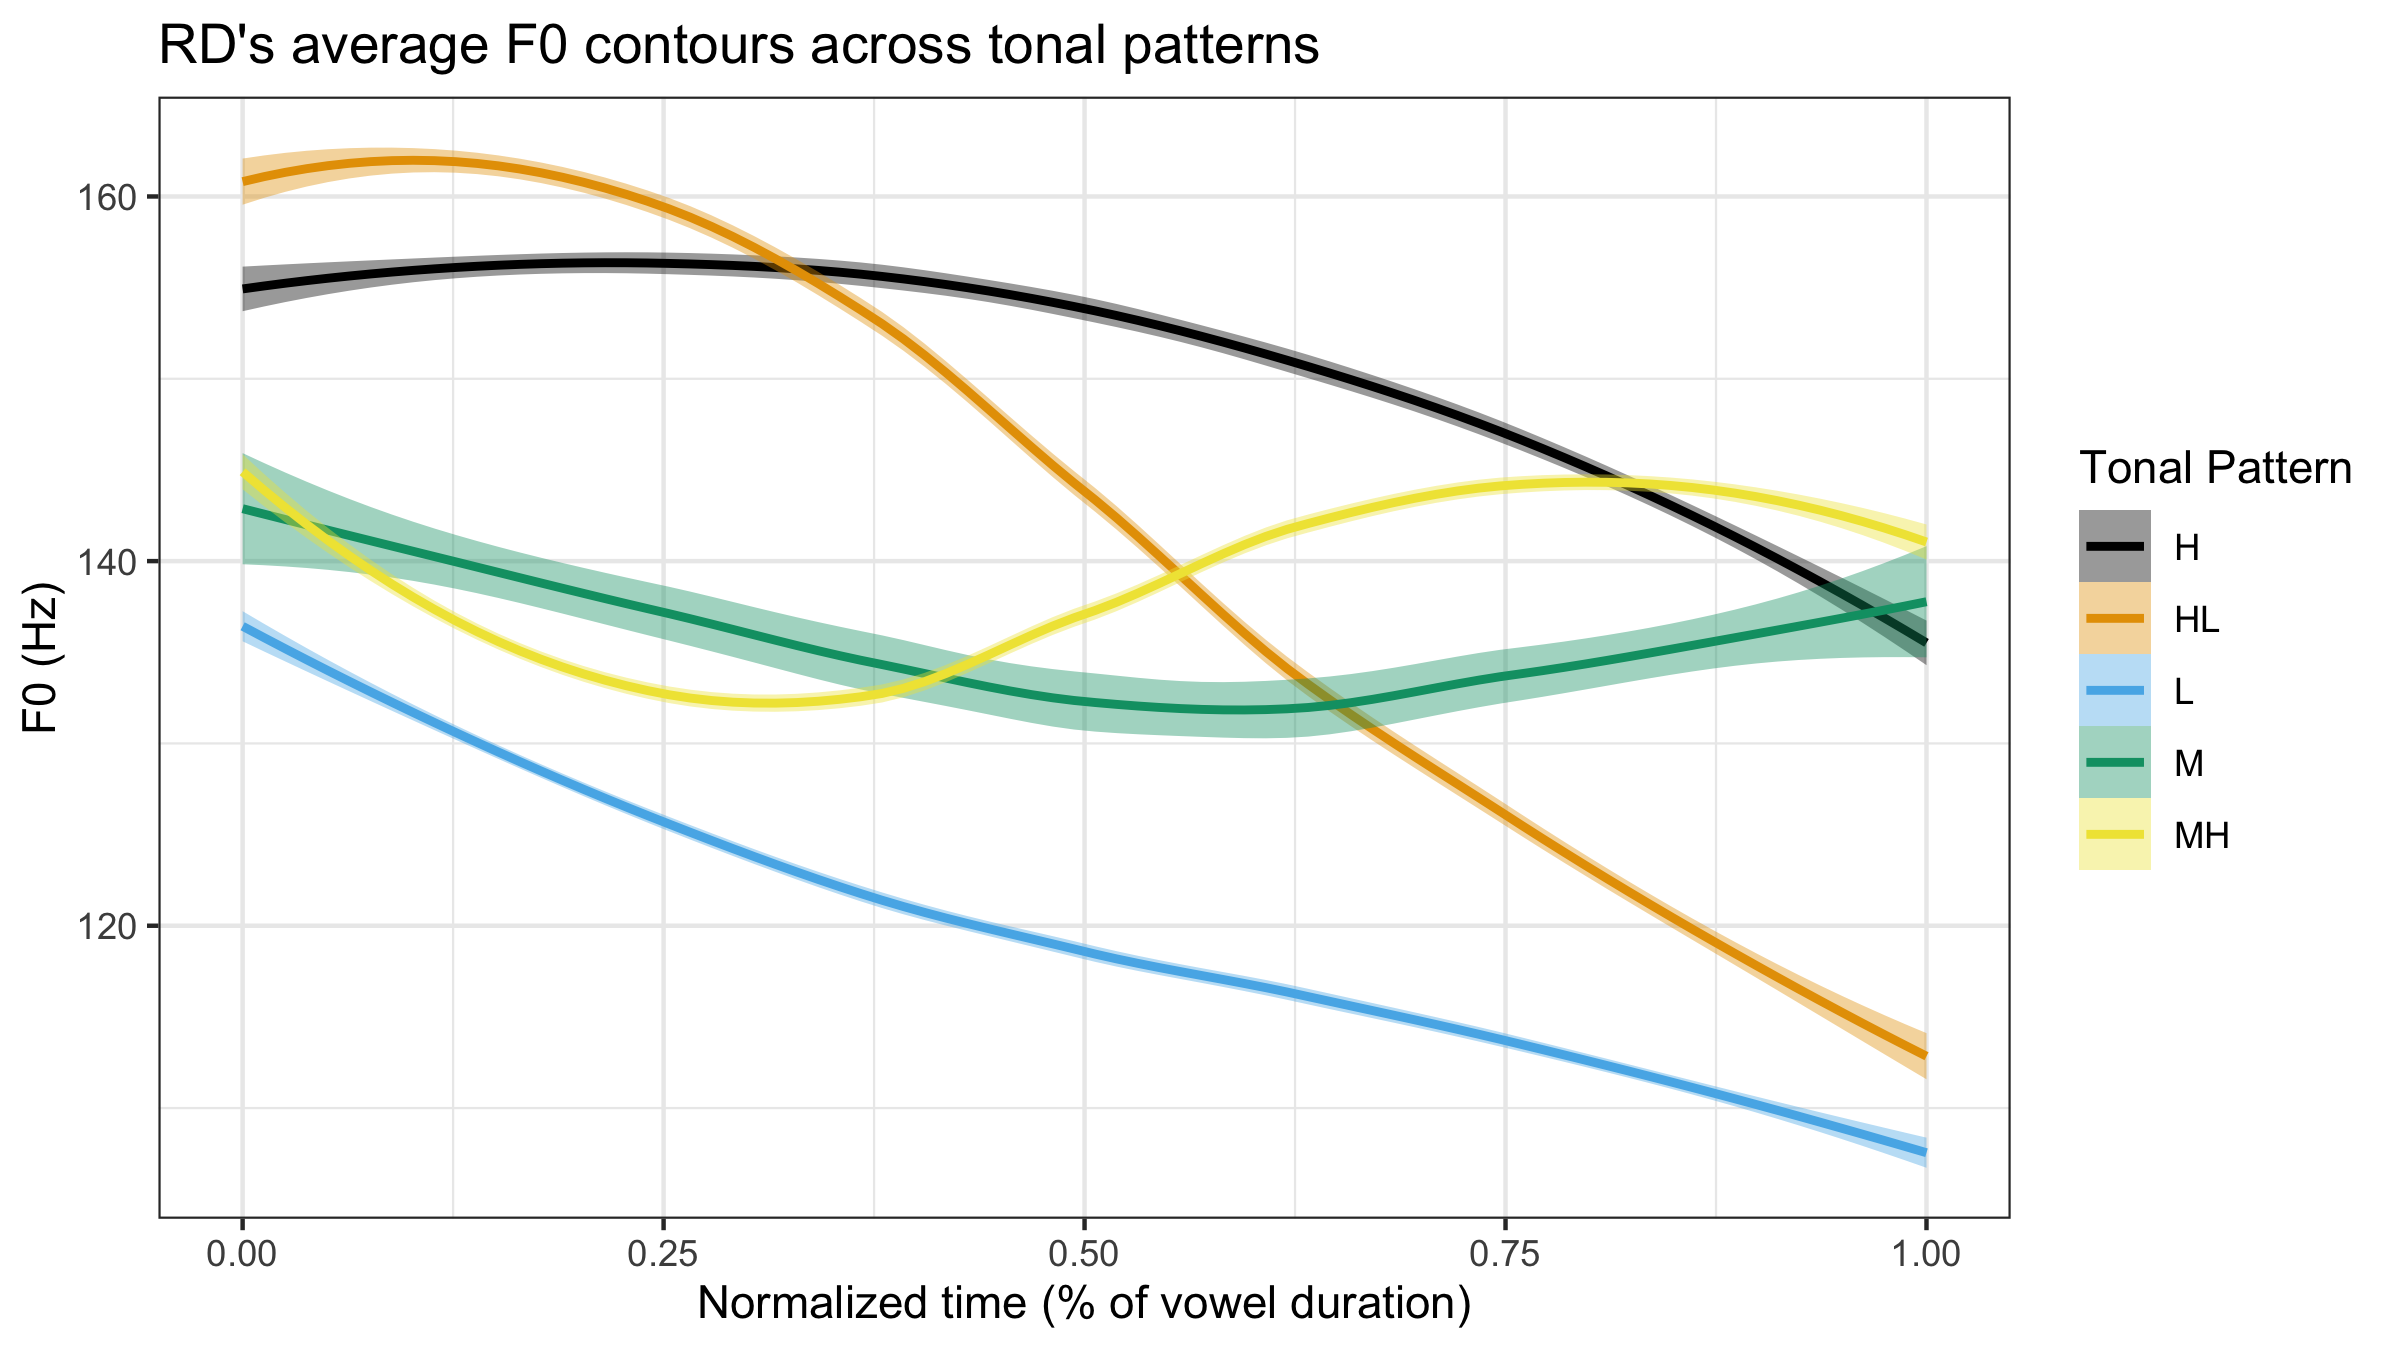
\includegraphics[width=0.9\textwidth]{../JoinTonePlot.png}
	\label{fig:LAMNetwork}
	\caption{Tonal contrasts for FSR and RD normalized for f0 and time.}
\end{figure}

%------------------------------------
\subsection{Phonation in SLZ} \label{sec:Phonation}
%------------------------------------

\begin{itemize}
	\item SLZ has four different contrastive phonation types on the vowels. 
	\begin{enumerate}
		\item Modal: [ a ] <\textit{a}>
		\item Breathy: [ a̤ ] <\textit{ah}> 
		\item Checked: [ aˀ ] <\textit{a'}> 
		\item Laryngealized: [ aˀa ] <\textit{a'a}> 
	\end{enumerate}
	\item Even though all of these contrastive phonation involve varying degrees of laryngealization, different configurations of the larynx, I choice to use the term laryngealized to refer to one of the phonation contrasts following the arguments from \citet{avelinoAcousticElectroglottographicAnalyses2010}.
	\begin{itemize}
		\item Laryngealized vowels do not have one consistent production of 
	\end{itemize}
\end{itemize}

%------------------------------------
\section{Interaction of Tone and Phonation} \label{sec:Interaction}
%------------------------------------

\begin{itemize}
	\item Table~\ref{tab:ToneVoiceQuality} shows the observed patterns between tone and phonation in SLZ. 
\end{itemize}

\vspace{-20pt}
\begin{table}[!h]
	\caption{Distribution of tone and voice quality in SLZ on a syllable}
	\label{tab:ToneVoiceQuality}
	\centering

	\begin{tabular}{lcccc}
	\hline

	\hline
		& \textbf{Modal} & \textbf{Breathy} & \textbf{Checked} & \textbf{Laryngealized} \\
	\hline
	H	& ✔ & -- & ✔ & ✔ \\
	M	& ✔ & ✔ & ✔ & ✔\\
	L	& ✔	& ✔ & ✔ & ✔\\
	HL	& ✔	& ✔ & ✔ & ✔\\
	MH	& ✔	& ✔ & -- & ✔ \\
	\hline

	\hline
	\end{tabular}
\end{table}

\begin{itemize}
	\item The striking observations that we find is that 
\end{itemize}
%------------------------------------
\section{Acoustic Measurements} \label{sec:Acoustics}
%------------------------------------

\begin{itemize}
	\item One way to investigate these interactions 
\end{itemize}

% \begin{figure}[]
% 	\includegraphics[width=0.9\textwidth]{../HA3_CheckedLaryngeal.png}
% 	\caption{}
%	\label{} 
% \end{figure}

% %------------------------------------
% \section{What's Next} \label{sec:Next}
% %------------------------------------

% %------------------------------------
% \section{What's Next} \label{sec:Next}
% %------------------------------------

% %------------------------------------
% \section{What's Next} \label{sec:Next}
% %------------------------------------

% %------------------------------------
% \section{What's Next} \label{sec:Next}
% %------------------------------------




% %------------------------------------
% \section{What's Next} \label{sec:Next}
% %------------------------------------



%------------------------------------
%BIBLIOGRAPHY
%------------------------------------

%\singlespacing
% \nocite{*}
\printbibliography[heading=bibintoc]

\end{document} 